\section{Stationery Envelope}

\begin{figure}[htbp]
\centering
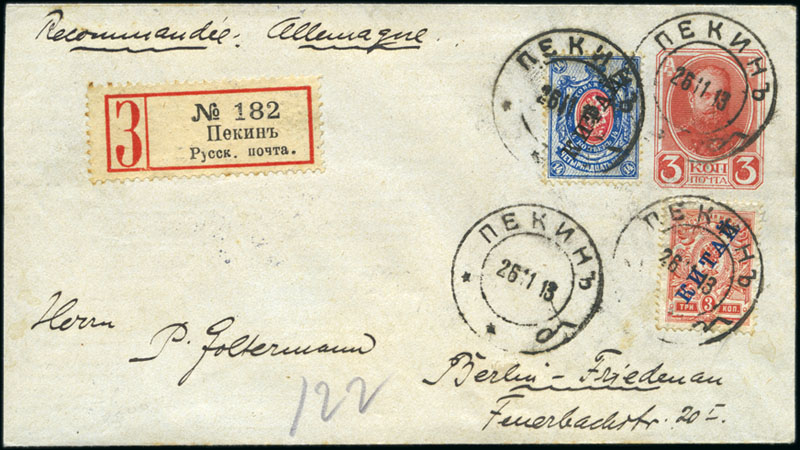
\includegraphics[width=.95\textwidth]{../russian-post-offices-in-china/10043.jpg}
\caption{
10043 PEKING: 1913 Romanov 3k postal stationery envelope registered to 
Germany, uprated with "KITAI" 3k and 14k paying the 10k foreign rate 
plus reg'n fee, all cancelled by Peking 26.11.13 cds (T\&S type 7B), 
with reg'd label in Cyrillic adjacent, a rare use of the Romanov stationery 
as ordinary Russian stamps and stationery wasn't sold in the 
Russian P.O.s in China.
\euro 300.00 
}  
\end{figure}   

Lorem ipsum dolor sit amet, consectetur adipiscing elit. Sed nibh justo, dictum sed cursus ac, lobortis et lacus. Vestibulum vitae justo enim. Quisque laoreet elementum felis, ut sodales arcu viverra a. Sed molestie odio vulputate sem rutrum a sagittis est rutrum. Morbi dapibus hendrerit magna, sit amet commodo massa posuere sit amet. Duis pharetra quam scelerisque est lobortis fringilla. Maecenas venenatis feugiat lectus, vel facilisis odio pharetra quis. Etiam at nisl eros, sit amet suscipit lorem. Lorem ipsum dolor sit amet, consectetur adipiscing elit. Sed augue nunc, ornare eget congue sit amet, laoreet vel augue. Morbi vel justo quis ipsum adipiscing egestas vitae non est. Vivamus ac quam quam. Nullam pharetra
                                                    interdum mauris, rutrum pulvinar ligula condimentum id. Donec et blandit lorem. 

\begin{figure}[htbp]
\centering
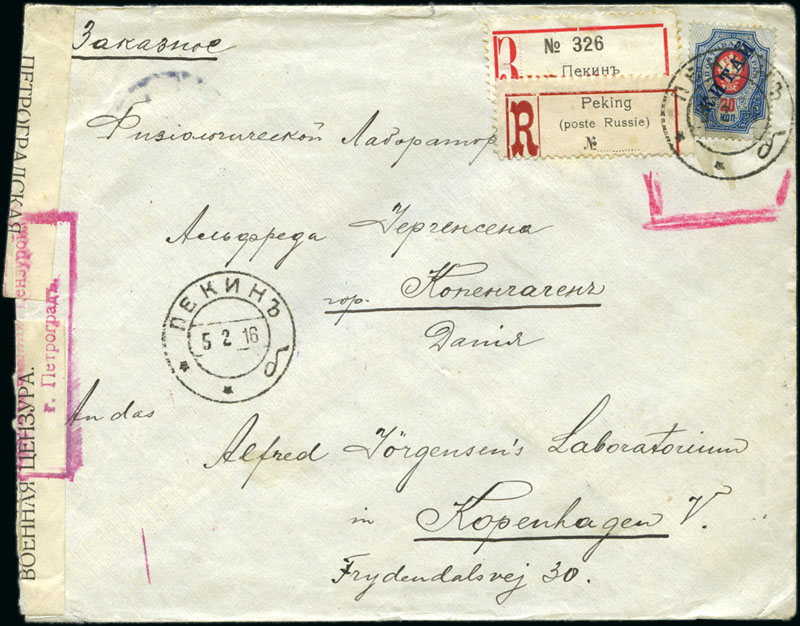
\includegraphics[width=.95\textwidth]{../russian-post-offices-in-china/10044.jpg}
\caption{
10044	PEKING: 1916 Cover registered to Denmark with 1899-1908 "KITAI" 
20k tied by Peking 5.2.16 cds (T\&S type 7B), opened and resealed by censor 
at Pertrograd, with reg'd labels in Cyrillic and French adjacent, with 
red crayon mark highlighting the use of an old issue and the possibility of 
fraudulent re-use, an interesting cover.
\euro 200.00 
}  
\end{figure}   


Lorem ipsum dolor sit amet, consectetur adipiscing elit. Sed nibh justo, dictum sed cursus ac, lobortis et lacus. Vestibulum vitae justo enim. Quisque laoreet elementum felis, ut sodales arcu viverra a. Sed molestie odio vulputate sem rutrum a sagittis est rutrum. Morbi dapibus hendrerit magna, sit amet commodo massa posuere sit amet. Duis pharetra quam scelerisque est lobortis fringilla. Maecenas venenatis feugiat lectus, vel facilisis odio pharetra quis. Etiam at nisl eros, sit amet suscipit lorem. Lorem ipsum dolor sit amet, consectetur adipiscing elit. Sed augue nunc, ornare eget congue sit amet, laoreet vel augue. Morbi vel justo quis ipsum adipiscing egestas vitae non est. Vivamus ac quam quam. Nullam pharetra
                                                    interdum mauris, rutrum pulvinar ligula condimentum id. Donec et blandit lorem. 

\clearpage

\begin{figure}[htbp]
\centering
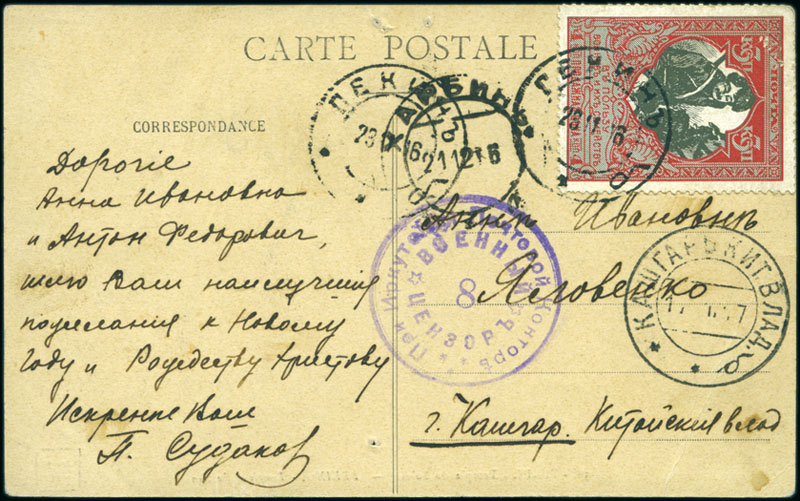
\includegraphics[width=.95\textwidth]{../russian-post-offices-in-china/10045.jpg}
\caption{
10045	PEKING: 1916 Picture postcard to Kashgar (SINKIANG) with 3k War 
Charity stamp tied by Peking 23.11.16 (T\&S type7B), sent via Harbin 
(Manchuria) and Irkutsk (Siberia) (where violet censor cachet was applied) 
with Kashgar 17.1.17 arrival cds, a very rare franking and route, showing 
re-entry into China
Note: War Charity stamps were not on sale in Russian P.O.s in China, but 
were accepted when supplied by the customer.
Note: Illustrated in "Russische Postcensuur 1914-1918" pg.23 by A. Speeckaert.
\euro 400.00. 
}  
\end{figure}   

\begin{figure}[htbp]
\centering
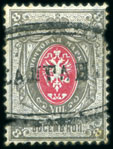
\includegraphics[width=.50\textwidth]{../russian-post-offices-in-china/10046.jpg}
\caption{
10046	KALGAN: 1875 8k Arms with dateless straight-line cancel in double 
oval (T\&S type 1), tiny thin at upper left otherwise fine and very rare.
Provenance: Ex Pappadopoulos, Blomfield and Torrey.
\euro 4,000.00 
}  
\end{figure}   


























                        